\section{Rozwój postaci gracza w grach (Bartosz Strzelecki, Bogna Lew)}\label{s:wpr_progres}
Rozwój postaci gracza ma ogromne znaczenie w wielu wymiarach. Jest podstawowym elementem, dzięki któremu gracz może odczuwać postęp podczas rozwoju linii fabularnych. 
Stanowi to też nagrodę dla gracza, za poniesioną głęboką osobistą inwestycję wczuwając się w rolę postaci. Przez to ta mechanika pozytywnie
wpływa na motywację użytkownika do dalszych zmagań i pozwala na ponowne rozegranie gry, dzięki temu, że gracz może chcieć przejść
ponownie przez linię fabularną, podejmując inne decyzje podczas rozwijania postaci.

Jednym z wyróżniających aspektów serii gier The Elder Scrolls jest zaimplementowany system rozwoju postaci, który pozwala na różnorodne
przebiegi rozgrywki dynamicznie dostosowujące się do stylu preferowanego przez gracza. W skrócie, jeśli gracz preferuje strzelanie z łuku,
w trakcie rozgrywki będzie mógł rozwijać tę umiejętność, aby czerpać z niej jak najwięcej korzyści. Głęboka złożoność tego systemu sprzyja długoterminowemu zaangażowaniu,
dzięki czemu gracze poświęcają dużo więcej czasu na doskonalenie swoich postaci, odkrywanie nowych kombinacji umiejętności i eksperymentowaniem z różnymi
stylami rozgrywki.

\begin{figure}[h]
\centering
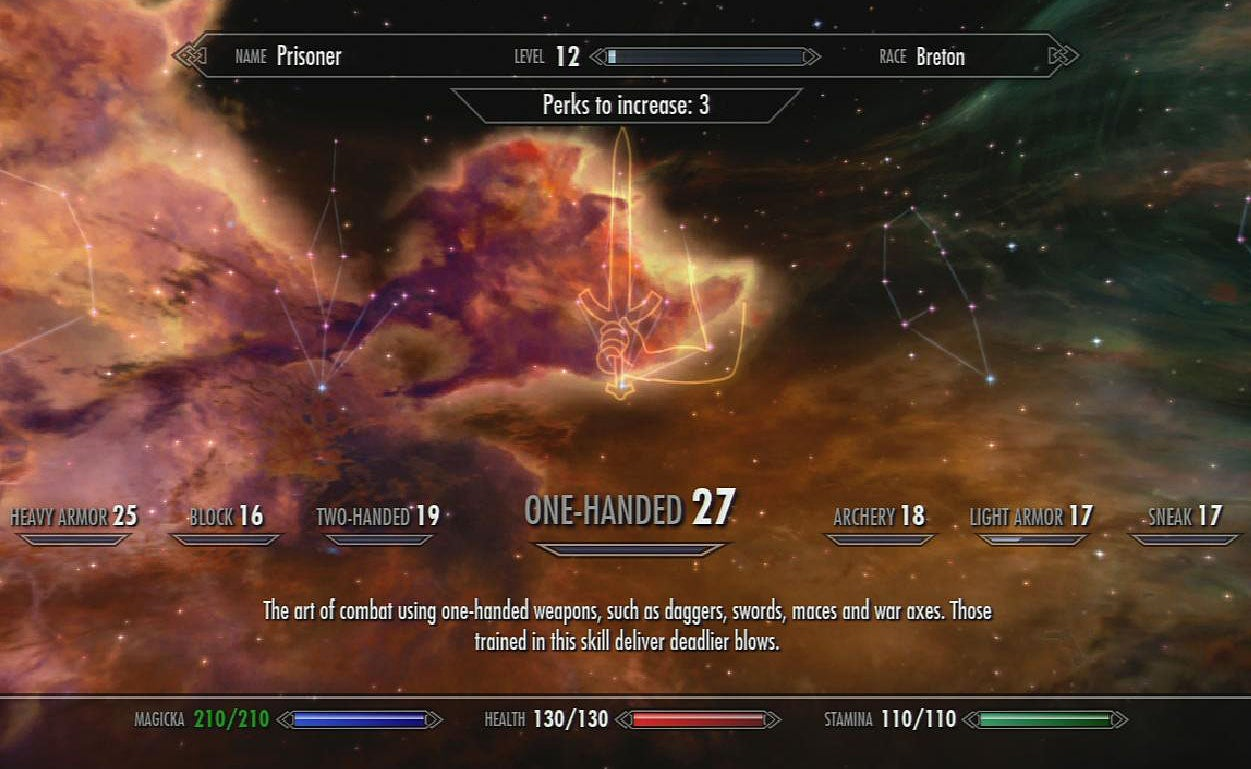
\includegraphics[width=1.0\textwidth]{images/tes.jpg}
\caption{Ekran rozwoju postaci z gry TESV: Skyrim.}
\end{figure}

Innym przykładem jest rozwój postaci w grze Wiedźmin 3: Dziki Gon, w której gracz wciela się w rolę wiedźmina Geralta.
Gra udostępnia cztery kategorie umiejętności bohatera, które użytkownik może rozwijać poprzez przyznawanie punktów. Gra
przyznaje je graczowi po tym jak zdobęcie on odpowiedni poziom doświadczenia, który może podnosić poprzez wykonywanie
zadań, czy zabijanie potworów. Każda z umiejętności, które gracz zdecyduje się rozwijać wymaga wcześniejszej aktywacji,
aby przynosić mu korzyści w trakcie rozgrywki. Jest to ciekawy mechanizm, który wymusza na graczu przemyślenie w jaki
sposób chce kształtować swoją postać i obmyślenie planu jej rozwoju.

\begin{figure}[h]
\centering
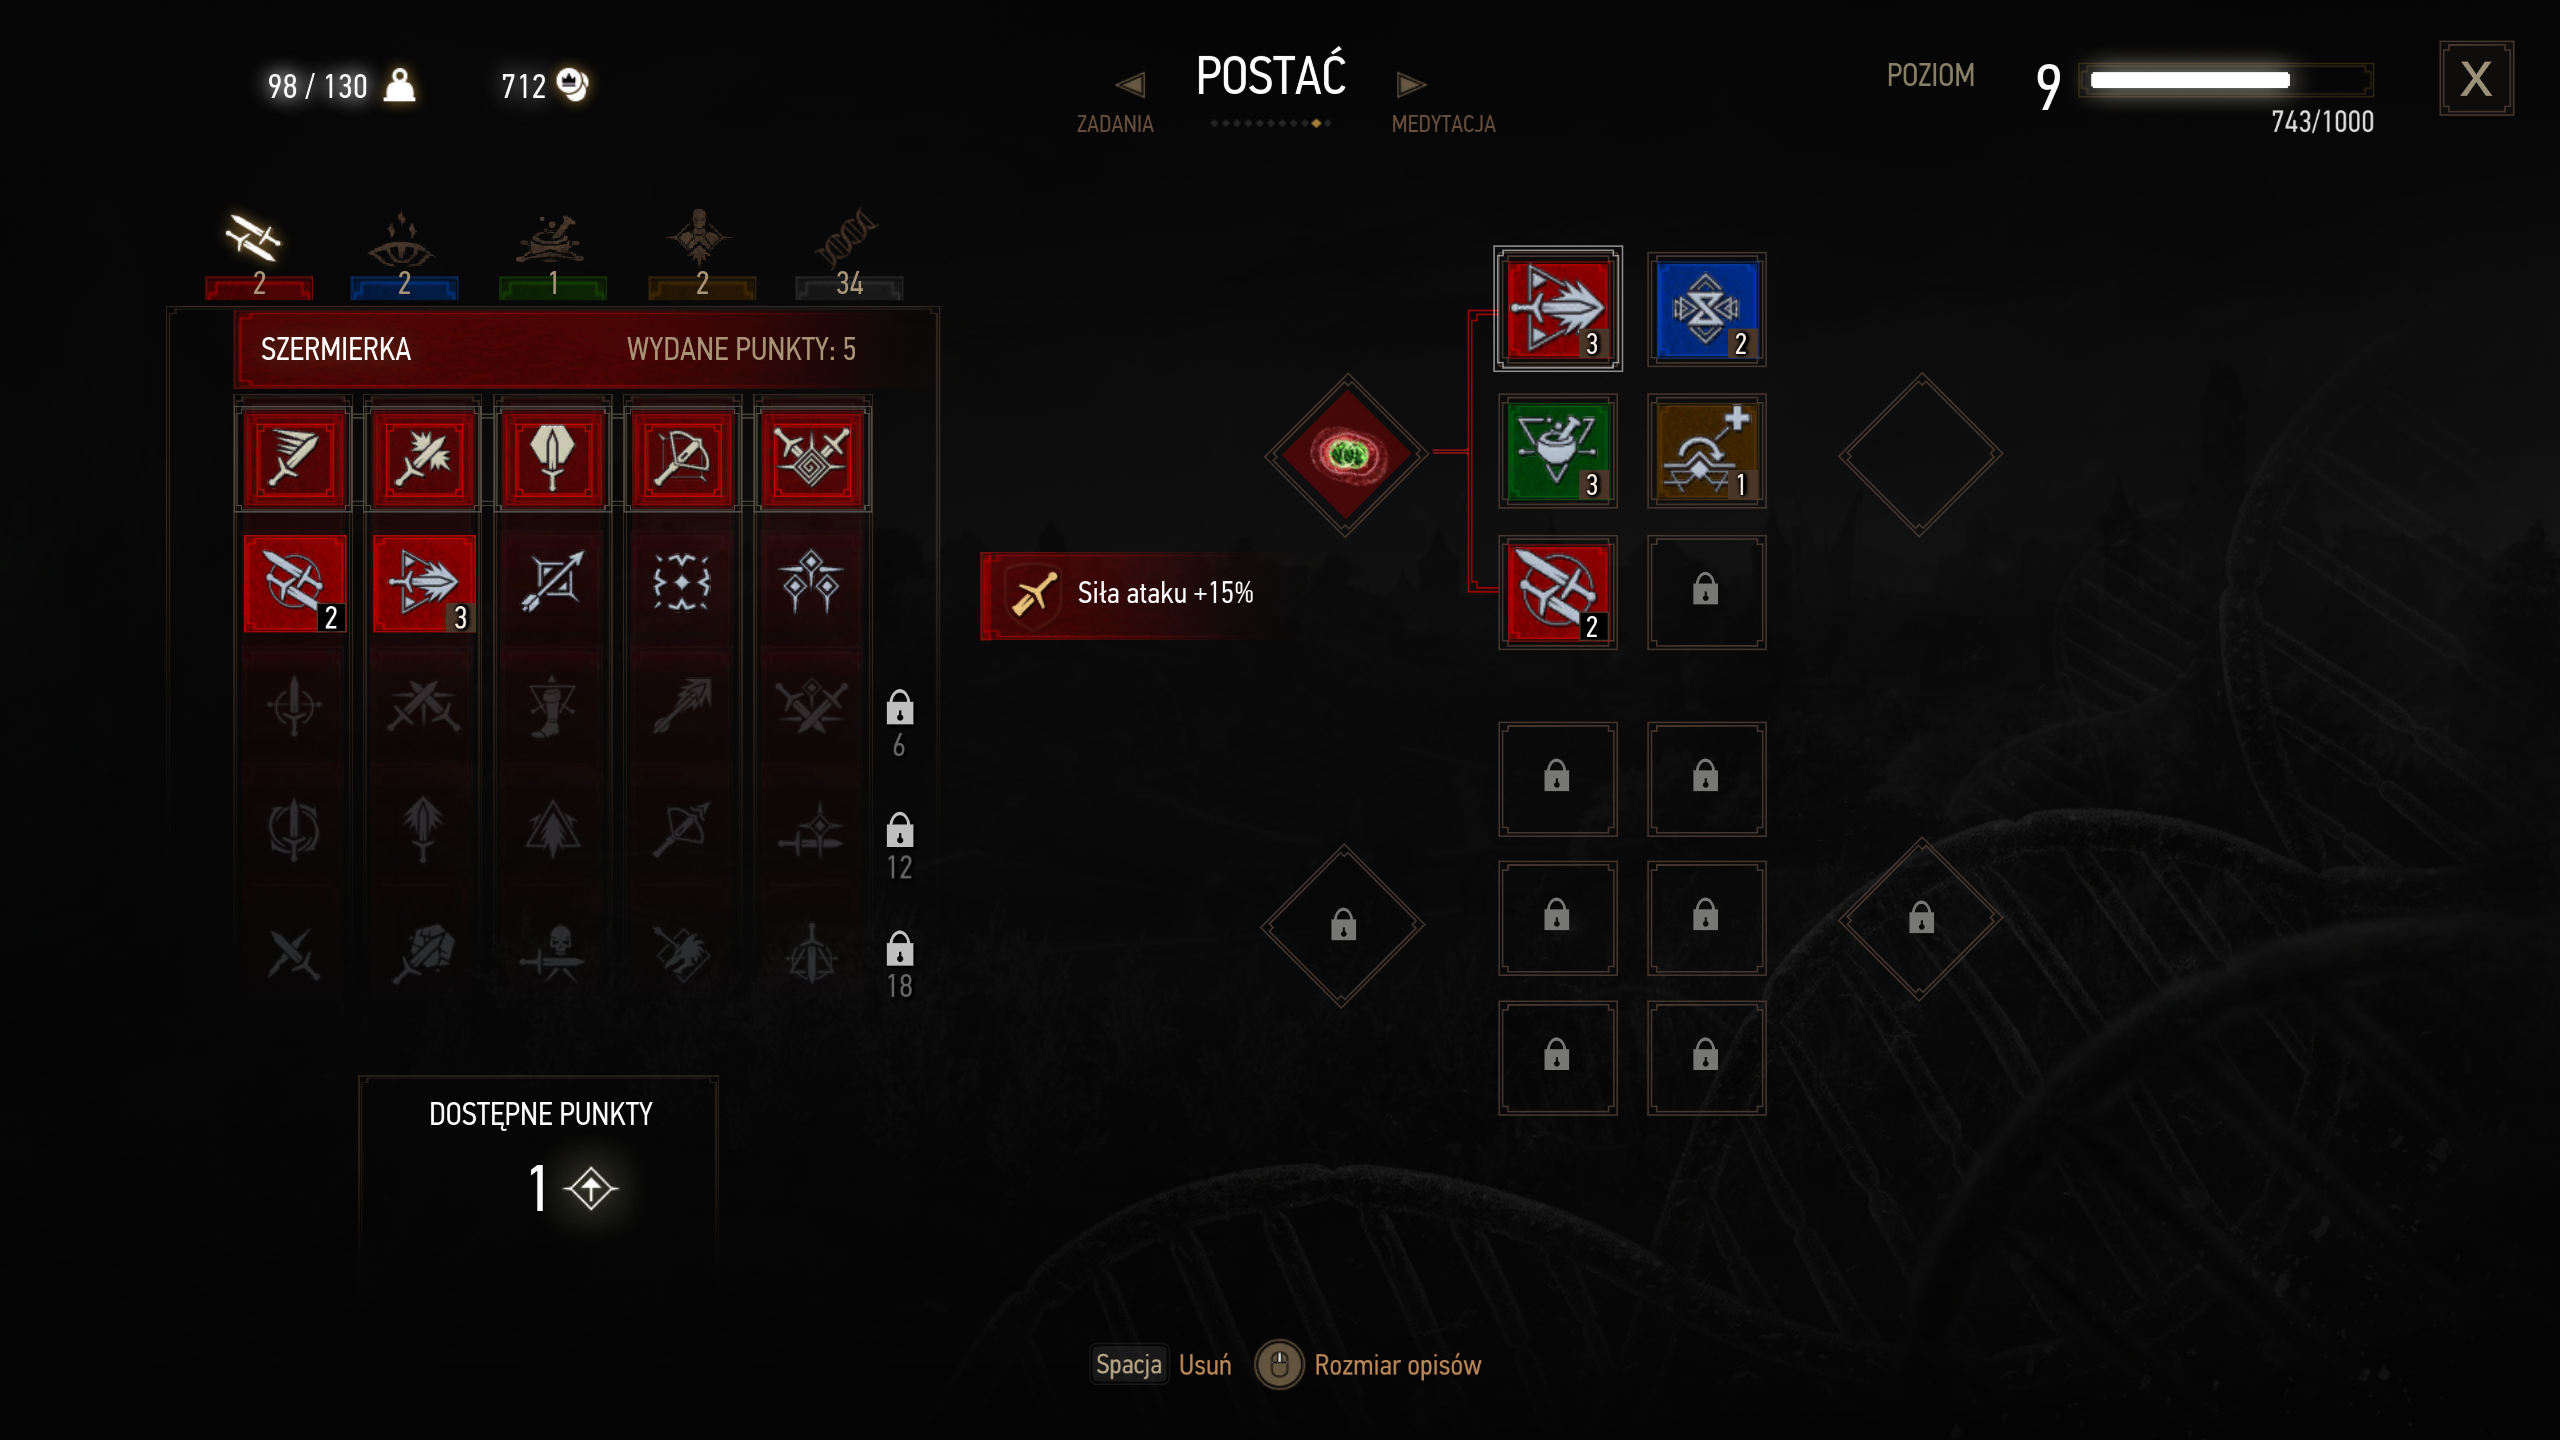
\includegraphics[width=1.0\textwidth]{images/wiedzmin.jpg}
\caption{Ekran rozwoju postaci z gry Wiedźmin 3: Dziki Gon.}
\end{figure}
